\documentclass[12pt]{article}

\usepackage[margin=0.8 in]{geometry}
\usepackage{amsmath}
\usepackage{amssymb}
\usepackage{macros}
\usepackage{mathtools}
\usepackage{enumerate}
\usepackage{verbatim}
\usepackage{amsthm}
\usepackage{hyperref}

\title{}
%\content{}



\let \proj \undefined
\renewcommand{\tr}{ \mathrm{tr}}
\DeclareMathOperator{\SU}{SU}
\DeclareMathOperator{\proj}{proj}
\newcommand{\sS}{\mathscr{S}}
\DeclareMathOperator{\comp}{comp}
\newcommand{\A}{\mathcal{A}}
\renewcommand{\D}{\mathcal{D}}
\renewcommand{\e}{\epsilon}
\newcommand{\et}{\tilde{\e}}
\newcommand{\vr}{\mathbf{r}}
\newcommand{\vF}{\mathbf{F}}
\newcommand{\triple}{\iiint_E f(x,y,z)dV}



\newenvironment{solution}
  {\begin{proof}[Solution]}
  {\end{proof}
  
  }
\newtheorem{example}{Example}
\newtheorem{exercise}{Exercise}
\newtheorem{theorem}{Theorem}
\newtheorem{definition}{Definition}


\begin{document}
\section*{Spherical coordinates}
What to know:
\begin{enumerate}
\item Change from Cartesian coordinates to Spherical and back
\item Be able to integrate in Spherical coordinates.
\end{enumerate}

\subsection*{Motivation and Relations}
Just like in the previous section, we'll see a coordinate system, that is, a method of describing points in the $xyz$ space in a manner that makes particular objects easily expressible. In cylindrical coordinates with respect to an axis, the corresponding objects were those with rotational symmetry about this axis; today it's going to be those with symmetry about the origin, such as spheres.
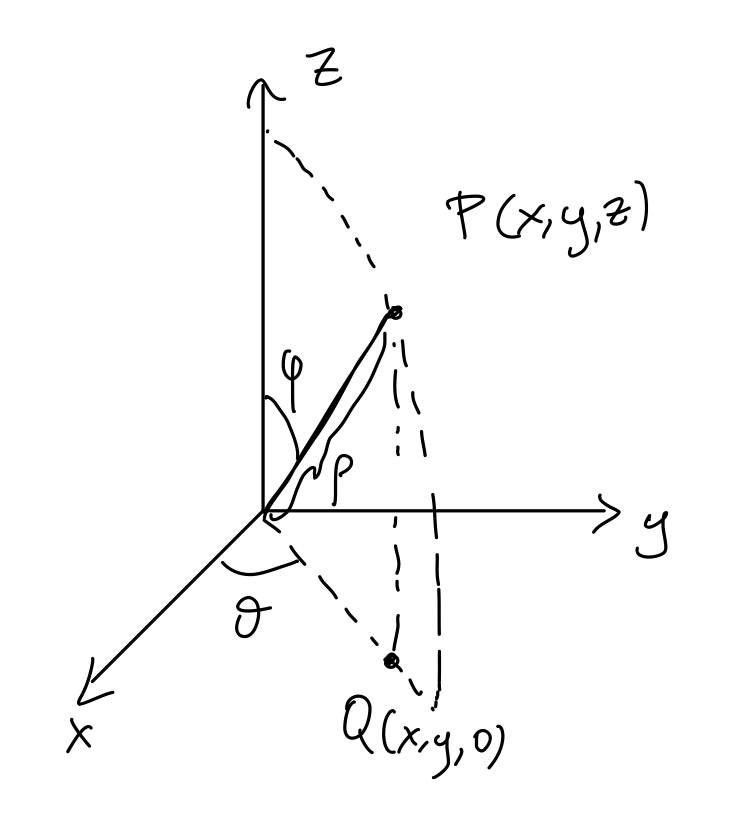
\includegraphics[scale=.2]{spherical.jpeg}
Say that we would like to describe a point $P(x,y,z)$ in coordinates $(\rho,\theta,\phi)$ so that spheres centered at the origin are as easily expressed as possible. Since a sphere centered at the origin is exactly the set of points whose distance from the origin is constant, it makes sense to set $\rho$ to be the distance from the origin, that is $$\rho=\sqrt{x^2+y^2+z^2}.$$ Then, if $O$ denotes the origin, we'll call $\phi$ the angle that $OP$ forms with the positive $z$ axis, which means that $$z=\rho \cos(\phi),$$ and we'll let it run from 0 to $\pi$.
Finally, in a similar way as with cylindrical coordinates, we'll project $P$ down to the $xy$ plane, call the projection $Q(x,y,0)$, and set $\theta$ to be the angle that the positive $x$ axis forms with $OQ$ (similar to polar coordinates), and let it run from 0 to $2\pi$. Note that, according to the definition we gave for $\rho $ and $\phi$, 	the distance of $Q$ from the origin is $\rho \sin(\phi)$. This means that, in the same way as with polar coordinates,
$$x=(\rho \sin(\phi))\cos(\theta)$$ and $$y=(\rho \sin(\phi))\sin(\theta).$$

Putting all these together, we find  

\[ \begin{matrix*}[l]%
&\rho =\sqrt{x^2+y^2+z^2}, 		\hspace{.5 in}						&\rho  \geq 0							\hspace{.5 in}					&x = \rho \sin(\phi)\cos(\theta)\\
&\cos(\phi) =\dfrac{z}{\sqrt{x^2+y^2+z^2}}, \hspace{.5 in}	&\phi  \in [0,\pi] 						\hspace{.5 in}					&y=\rho \sin(\phi)\sin(\theta)\\
&\tan(\theta) =\dfrac{y}{x}, 							\hspace{.5 in}		&\theta  \in [0,2\pi)		 			\hspace{.5 in}					&z=\rho \cos(\phi)
\end{matrix*}\]

\textbf{Remarks:}
\begin{enumerate}
\item We could allow for larger domains for $\rho, \phi$ and $\theta$ (assuming of course that we'd define $\rho$ by $\rho^2=x^2+y^2+z^2$ and not by its root). However, this would mean that a point would be expressible in multiple ways, just as in polar coordinates, so we usually pick the domains above\footnote{In fact, there is is still an issue with points that lie, for example, on the $z$ axis: The Cartesian point (0,0,$z_0$), $z_0>0$, can be written as ($z_0$, $\theta$,0) in spherical coordinates, for any $\theta$; if you want to be very careful you can define spherical coordinates on $\R^3$ except for the half plane $\{(x,0,z):x\geq 0\}$ to avoid this, but for the integration purposes we care about it's not going to make a difference and we won't worry about it too much.}.
\item Beware that the notation on spherical coordinates is generally nonstandard. That is, different authors might use different letters for spherical coordinates, or even define them differently (see the application at the end).
\end{enumerate}

\subsection*{Some surfaces in spherical coordinates}
As mentioned before, spherical coordinates are designed to make certain surfaces easy to express. A few examples:
\begin{enumerate}
\item The most typical example is a sphere of radius $c$ centered at the origin. It's written as $\rho=c$.
\item The equation $\theta= c$ denotes a half plane under the convention $0\leq \rho $ and $ 0\leq \phi \leq \pi$ (it would be a full plane if we allowed negative $\rho$ in our definition.
\item The equation $\phi = c$ is a half cone if $\phi \notin \{0,\frac{\pi}{2},\pi\}$. It becomes a half line for $\phi= 0 $ or $\pi$ and it coincides with the $xy$ plane for $\phi =\frac{\pi}{2}$.
\end{enumerate}

\textit{The surfaces above are visualized in a Mathematica file, here:} \url{http://sites.math.washington.edu/~neptamin/324Au17/Mathematica/}

\subsection*{Integration}
Since our topic of interest is integration, let's see how we integrate.

\begin{theorem}
Suppose that a solid $E$ is given in spherical coordinates as $$E=\{(\rho, \theta,\phi): \rho_1\leq \rho\leq \rho_2, \theta_1\leq \theta\leq \theta_2, \phi_1\leq\phi\leq\phi_2\}$$ and $f$ is a continuous function on $E$. Then
$$\triple =\int_{\rho_1}^{\rho_2}\int_{\theta_1}^{\theta_2}\int_{\phi_1}^{\phi_2}f(\rho \sin(\phi)\cos(\theta),\rho \sin(\phi)\sin(\theta),\rho \cos(\phi))\rho^2\sin(\phi)d\phi d\theta d\rho.$$
\end{theorem}

\begin{example}
Set up a triple integral in spherical coordinates for a function $f$ on a solid $E$, where $E$ is the solid bounded below by the cone $z=\sqrt{x^2+y^2}$ and bounded above by the sphere $x^2+y^2+z^2=25$.

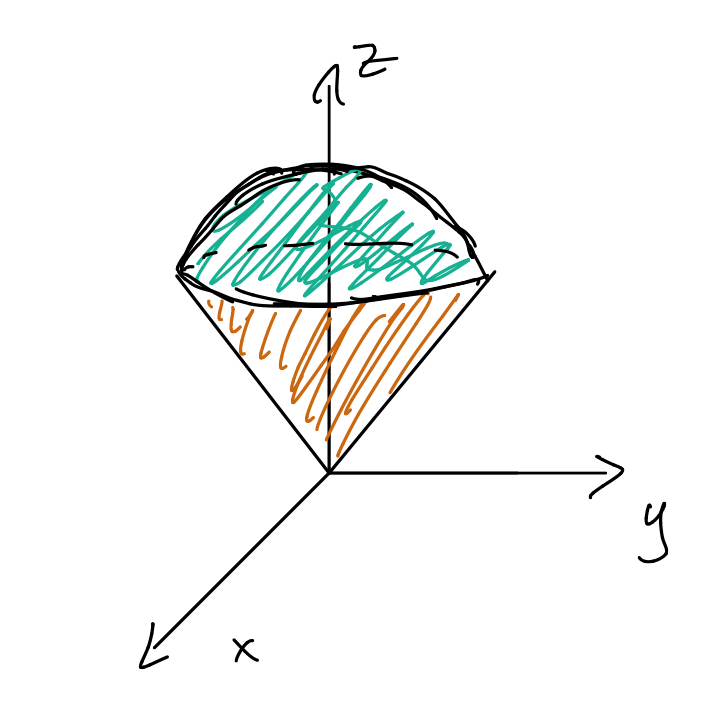
\includegraphics[scale=.2]{icecream.jpeg}

We write it in spherical coordinates: $$\sqrt{x^2+y^2}=z\implies \rho \sin(\phi)=\rho\cos(\phi)\implies \tan(\phi)=1\implies \phi=\frac{\pi}{4}.$$

So the fact that we're bounded below by the cone means that $$0\leq \phi\leq \frac{\pi}{4}.$$ The sphere can be written as $\rho=5$, so we also have $0\leq \rho\leq 5$. We have no restrictions on $\theta$, so $$0\leq \theta\leq 2\pi.$$ Finally $$\triple =\int_0^{2\pi}\int_0^{\frac{\pi}{4}}\int_0^5f(\rho \sin(\phi)\cos(\theta),\rho \sin(\phi)\sin(\theta),\rho \cos(\phi))\rho^2\sin(\phi)d\rho d\phi d\theta .$$

\end{example}

\subsection*{A real life application}
The coordinates used to describe points on the earth are a form of spherical coordinates. The \textbf{longitude} $\lambda$ stands for the angle east or west of the Prime Meridian that runs through Greenwich, UK and takes values in (-$180^\circ$, $180^\circ$). It corresponds to the $\theta$ we defined. The \textbf{latitude} measures the angle formed north or south of the equator, and takes values in (-$90^\circ$,$90^\circ$). It is analogous to our $\phi$, but $\phi$ measures angles from the positive $z$ axis instead.




\begin{center}
\begin{figure}
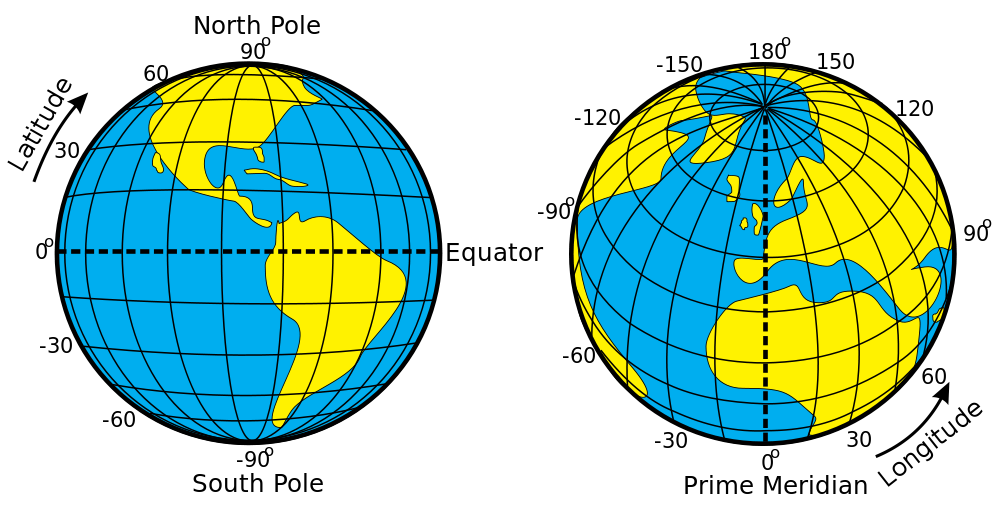
\includegraphics[scale=.3]{latitudelongitude.png}
\caption{Longitude and Latitude (picture from \url{http://www.geographyalltheway.com/ks3_geography/maps_atlases/longitude_latitude.htm}).}
\end{figure}
\end{center}


\end{document}

